\documentclass[twoside]{book}

% Packages required by doxygen
\usepackage{fixltx2e}
\usepackage{calc}
\usepackage{doxygen}
\usepackage[export]{adjustbox} % also loads graphicx
\usepackage{graphicx}
\usepackage[utf8]{inputenc}
\usepackage{makeidx}
\usepackage{multicol}
\usepackage{multirow}
\PassOptionsToPackage{warn}{textcomp}
\usepackage{textcomp}
\usepackage[nointegrals]{wasysym}
\usepackage[table]{xcolor}

% Font selection
\usepackage[T1]{fontenc}
\usepackage[scaled=.90]{helvet}
\usepackage{courier}
\usepackage{amssymb}
\usepackage{sectsty}
\renewcommand{\familydefault}{\sfdefault}
\allsectionsfont{%
  \fontseries{bc}\selectfont%
  \color{darkgray}%
}
\renewcommand{\DoxyLabelFont}{%
  \fontseries{bc}\selectfont%
  \color{darkgray}%
}
\newcommand{\+}{\discretionary{\mbox{\scriptsize$\hookleftarrow$}}{}{}}

% Page & text layout
\usepackage{geometry}
\geometry{%
  a4paper,%
  top=2.5cm,%
  bottom=2.5cm,%
  left=2.5cm,%
  right=2.5cm%
}
\tolerance=750
\hfuzz=15pt
\hbadness=750
\setlength{\emergencystretch}{15pt}
\setlength{\parindent}{0cm}
\setlength{\parskip}{3ex plus 2ex minus 2ex}
\makeatletter
\renewcommand{\paragraph}{%
  \@startsection{paragraph}{4}{0ex}{-1.0ex}{1.0ex}{%
    \normalfont\normalsize\bfseries\SS@parafont%
  }%
}
\renewcommand{\subparagraph}{%
  \@startsection{subparagraph}{5}{0ex}{-1.0ex}{1.0ex}{%
    \normalfont\normalsize\bfseries\SS@subparafont%
  }%
}
\makeatother

% Headers & footers
\usepackage{fancyhdr}
\pagestyle{fancyplain}
\fancyhead[LE]{\fancyplain{}{\bfseries\thepage}}
\fancyhead[CE]{\fancyplain{}{}}
\fancyhead[RE]{\fancyplain{}{\bfseries\leftmark}}
\fancyhead[LO]{\fancyplain{}{\bfseries\rightmark}}
\fancyhead[CO]{\fancyplain{}{}}
\fancyhead[RO]{\fancyplain{}{\bfseries\thepage}}
\fancyfoot[LE]{\fancyplain{}{}}
\fancyfoot[CE]{\fancyplain{}{}}
\fancyfoot[RE]{\fancyplain{}{\bfseries\scriptsize Generated by Doxygen }}
\fancyfoot[LO]{\fancyplain{}{\bfseries\scriptsize Generated by Doxygen }}
\fancyfoot[CO]{\fancyplain{}{}}
\fancyfoot[RO]{\fancyplain{}{}}
\renewcommand{\footrulewidth}{0.4pt}
\renewcommand{\chaptermark}[1]{%
  \markboth{#1}{}%
}
\renewcommand{\sectionmark}[1]{%
  \markright{\thesection\ #1}%
}

% Indices & bibliography
\usepackage{natbib}
\usepackage[titles]{tocloft}
\setcounter{tocdepth}{3}
\setcounter{secnumdepth}{5}
\makeindex

% Hyperlinks (required, but should be loaded last)
\usepackage{ifpdf}
\ifpdf
  \usepackage[pdftex,pagebackref=true]{hyperref}
\else
  \usepackage[ps2pdf,pagebackref=true]{hyperref}
\fi
\hypersetup{%
  colorlinks=true,%
  linkcolor=blue,%
  citecolor=blue,%
  unicode%
}

% Custom commands
\newcommand{\clearemptydoublepage}{%
  \newpage{\pagestyle{empty}\cleardoublepage}%
}

\usepackage{caption}
\captionsetup{labelsep=space,justification=centering,font={bf},singlelinecheck=off,skip=4pt,position=top}

%===== C O N T E N T S =====

\begin{document}

% Titlepage & ToC
\hypersetup{pageanchor=false,
             bookmarksnumbered=true,
             pdfencoding=unicode
            }
\pagenumbering{roman}
\begin{titlepage}
\vspace*{7cm}
\begin{center}%
{\Large Sof\+Ar Project }\\
\vspace*{1cm}
{\large Generated by Doxygen 1.8.11}\\
\end{center}
\end{titlepage}
\clearemptydoublepage
\tableofcontents
\clearemptydoublepage
\pagenumbering{arabic}
\hypersetup{pageanchor=true}

%--- Begin generated contents ---
\chapter{Class Index}
\section{Class List}
Here are the classes, structs, unions and interfaces with brief descriptions\+:\begin{DoxyCompactList}
\item\contentsline{section}{\hyperlink{classPclBackgroundSegmentation}{Pcl\+Background\+Segmentation} \\*Class to implement Background Segmentation }{\pageref{classPclBackgroundSegmentation}}{}
\item\contentsline{section}{\hyperlink{classPclFilter}{Pcl\+Filter} \\*Class to filter the Point Cloud }{\pageref{classPclFilter}}{}
\item\contentsline{section}{\hyperlink{classPclRecord}{Pcl\+Record} \\*Class to record environments }{\pageref{classPclRecord}}{}
\item\contentsline{section}{\hyperlink{classPoseEstimation}{Pose\+Estimation} \\*Class for estimating the Center of Mass }{\pageref{classPoseEstimation}}{}
\end{DoxyCompactList}

\chapter{File Index}
\section{File List}
Here is a list of all documented files with brief descriptions\+:\begin{DoxyCompactList}
\item\contentsline{section}{pose\+\_\+estimation/src/\hyperlink{pcl__background__segmentation_8cpp}{pcl\+\_\+background\+\_\+segmentation.\+cpp} \\*Main function\+: }{\pageref{pcl__background__segmentation_8cpp}}{}
\end{DoxyCompactList}

\chapter{Class Documentation}
\hypertarget{classPclBackgroundSegmentation}{}\section{Pcl\+Background\+Segmentation Class Reference}
\label{classPclBackgroundSegmentation}\index{Pcl\+Background\+Segmentation@{Pcl\+Background\+Segmentation}}


Class to implement Background Segmentation.  


\subsection*{Public Member Functions}
\begin{DoxyCompactItemize}
\item 
\hyperlink{classPclBackgroundSegmentation_a7e27a18fc9e7e7a0345d2ab0573b60bb}{Pcl\+Background\+Segmentation} ()
\item 
void \hyperlink{classPclBackgroundSegmentation_adc1a5bace5ac90646ff552336564acbc}{back\+CB} (const sensor\+\_\+msgs\+::\+Point\+Cloud2 \&input)
\item 
void \hyperlink{classPclBackgroundSegmentation_a2255df663f6848dc6a59e6d31f058c0b}{angle\+CB} (const std\+\_\+msgs\+::\+Float64 \&angle\+\_\+msg)
\end{DoxyCompactItemize}
\subsection*{Protected Attributes}
\begin{DoxyCompactItemize}
\item 
ros\+::\+Node\+Handle {\bfseries nh}\hypertarget{classPclBackgroundSegmentation_a42e22fca2c30a57d35b09d5077279cca}{}\label{classPclBackgroundSegmentation_a42e22fca2c30a57d35b09d5077279cca}

\item 
ros\+::\+Subscriber {\bfseries pcl\+\_\+sub}\hypertarget{classPclBackgroundSegmentation_a48bba168a2eb4c6521dd77110d71f1f4}{}\label{classPclBackgroundSegmentation_a48bba168a2eb4c6521dd77110d71f1f4}

\item 
ros\+::\+Subscriber {\bfseries angle\+\_\+sub}\hypertarget{classPclBackgroundSegmentation_a4137ec77c2ed7ce6aa01b9ed6ca6891a}{}\label{classPclBackgroundSegmentation_a4137ec77c2ed7ce6aa01b9ed6ca6891a}

\item 
ros\+::\+Publisher {\bfseries pcl\+\_\+pub}\hypertarget{classPclBackgroundSegmentation_a9ac6a20a2cd1c05cb74db86e967bc074}{}\label{classPclBackgroundSegmentation_a9ac6a20a2cd1c05cb74db86e967bc074}

\end{DoxyCompactItemize}


\subsection{Detailed Description}
Class to implement Background Segmentation. 

The class removes the background, associated to the current Kinect angle, from the raw Point Cloud acquired by the Kinect and saved in /camera/depth/points. The filtered point cloud is published on the topic /camera/pcl\+\_\+background\+\_\+segmentation 

\subsection{Constructor \& Destructor Documentation}
\index{Pcl\+Background\+Segmentation@{Pcl\+Background\+Segmentation}!Pcl\+Background\+Segmentation@{Pcl\+Background\+Segmentation}}
\index{Pcl\+Background\+Segmentation@{Pcl\+Background\+Segmentation}!Pcl\+Background\+Segmentation@{Pcl\+Background\+Segmentation}}
\subsubsection[{\texorpdfstring{Pcl\+Background\+Segmentation()}{PclBackgroundSegmentation()}}]{\setlength{\rightskip}{0pt plus 5cm}Pcl\+Background\+Segmentation\+::\+Pcl\+Background\+Segmentation (
\begin{DoxyParamCaption}
{}
\end{DoxyParamCaption}
)\hspace{0.3cm}{\ttfamily [inline]}}\hypertarget{classPclBackgroundSegmentation_a7e27a18fc9e7e7a0345d2ab0573b60bb}{}\label{classPclBackgroundSegmentation_a7e27a18fc9e7e7a0345d2ab0573b60bb}
Handler\+:
\begin{DoxyItemize}
\item subscribe to /camera/depth/points to get raw data acquired by the Kinect
\item subscribe to /cur\+\_\+tilt\+\_\+angle to know the current tilt angle of the Kinect
\item publish filtered point cloud on /camera/pcl\+\_\+background\+\_\+segmentation 
\end{DoxyItemize}

\subsection{Member Function Documentation}
\index{Pcl\+Background\+Segmentation@{Pcl\+Background\+Segmentation}!angle\+CB@{angle\+CB}}
\index{angle\+CB@{angle\+CB}!Pcl\+Background\+Segmentation@{Pcl\+Background\+Segmentation}}
\subsubsection[{\texorpdfstring{angle\+C\+B(const std\+\_\+msgs\+::\+Float64 \&angle\+\_\+msg)}{angleCB(const std_msgs::Float64 &angle_msg)}}]{\setlength{\rightskip}{0pt plus 5cm}void Pcl\+Background\+Segmentation\+::angle\+CB (
\begin{DoxyParamCaption}
\item[{const std\+\_\+msgs\+::\+Float64 \&}]{angle\+\_\+msg}
\end{DoxyParamCaption}
)\hspace{0.3cm}{\ttfamily [inline]}}\hypertarget{classPclBackgroundSegmentation_a2255df663f6848dc6a59e6d31f058c0b}{}\label{classPclBackgroundSegmentation_a2255df663f6848dc6a59e6d31f058c0b}
Angle callback function acquires the current tilt angle of the Kinect that is useful to know the right background to remove 
\begin{DoxyParams}[1]{Parameters}
\mbox{\tt in}  & {\em angle\+\_\+msg} & current tilt angle of the Kinect \\
\hline
\end{DoxyParams}
\index{Pcl\+Background\+Segmentation@{Pcl\+Background\+Segmentation}!back\+CB@{back\+CB}}
\index{back\+CB@{back\+CB}!Pcl\+Background\+Segmentation@{Pcl\+Background\+Segmentation}}
\subsubsection[{\texorpdfstring{back\+C\+B(const sensor\+\_\+msgs\+::\+Point\+Cloud2 \&input)}{backCB(const sensor_msgs::PointCloud2 &input)}}]{\setlength{\rightskip}{0pt plus 5cm}void Pcl\+Background\+Segmentation\+::back\+CB (
\begin{DoxyParamCaption}
\item[{const sensor\+\_\+msgs\+::\+Point\+Cloud2 \&}]{input}
\end{DoxyParamCaption}
)\hspace{0.3cm}{\ttfamily [inline]}}\hypertarget{classPclBackgroundSegmentation_adc1a5bace5ac90646ff552336564acbc}{}\label{classPclBackgroundSegmentation_adc1a5bace5ac90646ff552336564acbc}
Point cloud callback function\+:
\begin{DoxyItemize}
\item remove the background associated to the current Kinect angle from the /camera/depth/points
\item publish filtered points cloud in /camera/pcl\+\_\+background\+\_\+segmentation 
\begin{DoxyParams}[1]{Parameters}
\mbox{\tt in}  & {\em input} & point cloud data from the Kinect \\
\hline
\end{DoxyParams}

\end{DoxyItemize}

The documentation for this class was generated from the following file\+:\begin{DoxyCompactItemize}
\item 
pose\+\_\+estimation/src/pcl\+\_\+background\+\_\+segmentation.\+cpp\end{DoxyCompactItemize}

\hypertarget{classPclFilter}{}\section{Pcl\+Filter Class Reference}
\label{classPclFilter}\index{Pcl\+Filter@{Pcl\+Filter}}


Class to filter the Point Cloud.  


\subsection*{Public Member Functions}
\begin{DoxyCompactItemize}
\item 
\hyperlink{classPclFilter_a6fdc19ebc1821b00c7becccd251e010a}{Pcl\+Filter} ()
\item 
void \hyperlink{classPclFilter_a2f12ba73fa3b2c3a97978d20ea7909d1}{filter\+CB} (const boost\+::shared\+\_\+ptr$<$ const sensor\+\_\+msgs\+::\+Point\+Cloud2 $>$ \&input)
\end{DoxyCompactItemize}
\subsection*{Protected Attributes}
\begin{DoxyCompactItemize}
\item 
ros\+::\+Node\+Handle {\bfseries nh}\hypertarget{classPclFilter_a0777606b8bbca26a783c1276405b0256}{}\label{classPclFilter_a0777606b8bbca26a783c1276405b0256}

\item 
ros\+::\+Subscriber {\bfseries pcl\+\_\+sub}\hypertarget{classPclFilter_a553c3349ea2f3a5d890893cf8dcf5352}{}\label{classPclFilter_a553c3349ea2f3a5d890893cf8dcf5352}

\item 
ros\+::\+Publisher {\bfseries pcl\+\_\+pub}\hypertarget{classPclFilter_afa21edff9a4d7cdd6f1bd1f02d819eee}{}\label{classPclFilter_afa21edff9a4d7cdd6f1bd1f02d819eee}

\end{DoxyCompactItemize}
\subsection*{Private Attributes}
\begin{DoxyCompactItemize}
\item 
pcl\+::\+Point\+Cloud$<$ pcl\+::\+Point\+X\+YZ $>$ \hyperlink{classPclFilter_af18d36d2d1c3fcbba45be49a32ae9e11}{cloud}
\item 
pcl\+::\+Point\+Cloud$<$ pcl\+::\+Point\+X\+YZ $>$ \hyperlink{classPclFilter_a06aae25878fdd6c3aad05fa00f4c0f07}{cloud\+\_\+filtered}
\item 
pcl\+::\+Statistical\+Outlier\+Removal$<$ pcl\+::\+Point\+X\+YZ $>$ \hyperlink{classPclFilter_a8e402978eb3fdedcbee54554fe55c259}{stat\+Filter}
\end{DoxyCompactItemize}


\subsection{Detailed Description}
Class to filter the Point Cloud. 

The class has the aim of filtering the Point Cloud obtained by the background segmentation and saved in /camera/pcl\+\_\+background\+\_\+segmentation. It uses different filters\+:
\begin{DoxyItemize}
\item Downsampling (with Voxel\+Grid)
\item X\+YZ axes range filter
\item Statistical Outlier Removal Filter and publish the filtered point cloud on /camera/pcl\+\_\+filtered 
\end{DoxyItemize}

\subsection{Constructor \& Destructor Documentation}
\index{Pcl\+Filter@{Pcl\+Filter}!Pcl\+Filter@{Pcl\+Filter}}
\index{Pcl\+Filter@{Pcl\+Filter}!Pcl\+Filter@{Pcl\+Filter}}
\subsubsection[{\texorpdfstring{Pcl\+Filter()}{PclFilter()}}]{\setlength{\rightskip}{0pt plus 5cm}Pcl\+Filter\+::\+Pcl\+Filter (
\begin{DoxyParamCaption}
{}
\end{DoxyParamCaption}
)\hspace{0.3cm}{\ttfamily [inline]}}\hypertarget{classPclFilter_a6fdc19ebc1821b00c7becccd251e010a}{}\label{classPclFilter_a6fdc19ebc1821b00c7becccd251e010a}
Handler\+:
\begin{DoxyItemize}
\item subscribe to /camera/pcl\+\_\+background\+\_\+segmentation to get the point cloud obtained by the background segmentation
\item publish filtered point cloud on /camera/pcl\+\_\+filtered 
\end{DoxyItemize}

\subsection{Member Function Documentation}
\index{Pcl\+Filter@{Pcl\+Filter}!filter\+CB@{filter\+CB}}
\index{filter\+CB@{filter\+CB}!Pcl\+Filter@{Pcl\+Filter}}
\subsubsection[{\texorpdfstring{filter\+C\+B(const boost\+::shared\+\_\+ptr$<$ const sensor\+\_\+msgs\+::\+Point\+Cloud2 $>$ \&input)}{filterCB(const boost::shared_ptr< const sensor_msgs::PointCloud2 > &input)}}]{\setlength{\rightskip}{0pt plus 5cm}void Pcl\+Filter\+::filter\+CB (
\begin{DoxyParamCaption}
\item[{const boost\+::shared\+\_\+ptr$<$ const sensor\+\_\+msgs\+::\+Point\+Cloud2 $>$ \&}]{input}
\end{DoxyParamCaption}
)\hspace{0.3cm}{\ttfamily [inline]}}\hypertarget{classPclFilter_a2f12ba73fa3b2c3a97978d20ea7909d1}{}\label{classPclFilter_a2f12ba73fa3b2c3a97978d20ea7909d1}
Callback function implementation of filters\+:
\begin{DoxyItemize}
\item Downsampling filter with parameter leaf\+\_\+size
\item Filter on z axis in range (min\+\_\+z, max\+\_\+z)
\item Filter on x axis in range (min\+\_\+x, max\+\_\+x)
\item Filter on y axis in range (min\+\_\+y, max\+\_\+y)
\item Statistical Outlier Removal filter to remove outliers 
\begin{DoxyParams}[1]{Parameters}
\mbox{\tt in}  & {\em input} & point cloud data from background segmentation \\
\hline
\end{DoxyParams}

\end{DoxyItemize}

\subsection{Member Data Documentation}
\index{Pcl\+Filter@{Pcl\+Filter}!cloud@{cloud}}
\index{cloud@{cloud}!Pcl\+Filter@{Pcl\+Filter}}
\subsubsection[{\texorpdfstring{cloud}{cloud}}]{\setlength{\rightskip}{0pt plus 5cm}pcl\+::\+Point\+Cloud$<$pcl\+::\+Point\+X\+YZ$>$ Pcl\+Filter\+::cloud\hspace{0.3cm}{\ttfamily [private]}}\hypertarget{classPclFilter_af18d36d2d1c3fcbba45be49a32ae9e11}{}\label{classPclFilter_af18d36d2d1c3fcbba45be49a32ae9e11}
Input Point Cloud \index{Pcl\+Filter@{Pcl\+Filter}!cloud\+\_\+filtered@{cloud\+\_\+filtered}}
\index{cloud\+\_\+filtered@{cloud\+\_\+filtered}!Pcl\+Filter@{Pcl\+Filter}}
\subsubsection[{\texorpdfstring{cloud\+\_\+filtered}{cloud_filtered}}]{\setlength{\rightskip}{0pt plus 5cm}pcl\+::\+Point\+Cloud$<$pcl\+::\+Point\+X\+YZ$>$ Pcl\+Filter\+::cloud\+\_\+filtered\hspace{0.3cm}{\ttfamily [private]}}\hypertarget{classPclFilter_a06aae25878fdd6c3aad05fa00f4c0f07}{}\label{classPclFilter_a06aae25878fdd6c3aad05fa00f4c0f07}
Output Point Cloud \index{Pcl\+Filter@{Pcl\+Filter}!stat\+Filter@{stat\+Filter}}
\index{stat\+Filter@{stat\+Filter}!Pcl\+Filter@{Pcl\+Filter}}
\subsubsection[{\texorpdfstring{stat\+Filter}{statFilter}}]{\setlength{\rightskip}{0pt plus 5cm}pcl\+::\+Statistical\+Outlier\+Removal$<$pcl\+::\+Point\+X\+YZ$>$ Pcl\+Filter\+::stat\+Filter\hspace{0.3cm}{\ttfamily [private]}}\hypertarget{classPclFilter_a8e402978eb3fdedcbee54554fe55c259}{}\label{classPclFilter_a8e402978eb3fdedcbee54554fe55c259}
Statistical Outlier Removal Filter 

The documentation for this class was generated from the following file\+:\begin{DoxyCompactItemize}
\item 
pose\+\_\+estimation/src/pcl\+\_\+filter.\+cpp\end{DoxyCompactItemize}

\hypertarget{classPclRecord}{}\section{Pcl\+Record Class Reference}
\label{classPclRecord}\index{Pcl\+Record@{Pcl\+Record}}


Class to record environments.  


\subsection*{Public Member Functions}
\begin{DoxyCompactItemize}
\item 
\hyperlink{classPclRecord_adcde62c71c552ef09800920d24e313e2}{Pcl\+Record} ()
\item 
void \hyperlink{classPclRecord_a19c604de9fbe99982ed880c5556a429b}{Pcl\+Record\+CB} (const sensor\+\_\+msgs\+::\+Point\+Cloud2\+Const\+Ptr \&cloud)
\item 
void {\bfseries Angle\+CB} (const std\+\_\+msgs\+::\+Float64 msg\+\_\+angle)\hypertarget{classPclRecord_afd60b0301ae3d8a4b00e29d195d4345d}{}\label{classPclRecord_afd60b0301ae3d8a4b00e29d195d4345d}

\end{DoxyCompactItemize}
\subsection*{Protected Attributes}
\begin{DoxyCompactItemize}
\item 
ros\+::\+Node\+Handle {\bfseries nh}\hypertarget{classPclRecord_acdce8386b8daeb1d3a5da49b0e1acf41}{}\label{classPclRecord_acdce8386b8daeb1d3a5da49b0e1acf41}

\item 
ros\+::\+Subscriber {\bfseries pcl\+\_\+sub}\hypertarget{classPclRecord_ada2acf1a126c6b6ad0593ded229321df}{}\label{classPclRecord_ada2acf1a126c6b6ad0593ded229321df}

\item 
ros\+::\+Subscriber {\bfseries angle\+\_\+sub}\hypertarget{classPclRecord_a26421aa8c5e60cf4561aba798ea8623f}{}\label{classPclRecord_a26421aa8c5e60cf4561aba798ea8623f}

\end{DoxyCompactItemize}


\subsection{Detailed Description}
Class to record environments. 

The class records all the environments for each possible orientation of the Kinect
\begin{DoxyItemize}
\item the range of the Kinect tilt is \mbox{[}-\/30,30\mbox{]} degree
\item acquisitions with a given granularity 
\end{DoxyItemize}

\subsection{Constructor \& Destructor Documentation}
\index{Pcl\+Record@{Pcl\+Record}!Pcl\+Record@{Pcl\+Record}}
\index{Pcl\+Record@{Pcl\+Record}!Pcl\+Record@{Pcl\+Record}}
\subsubsection[{\texorpdfstring{Pcl\+Record()}{PclRecord()}}]{\setlength{\rightskip}{0pt plus 5cm}Pcl\+Record\+::\+Pcl\+Record (
\begin{DoxyParamCaption}
{}
\end{DoxyParamCaption}
)\hspace{0.3cm}{\ttfamily [inline]}}\hypertarget{classPclRecord_adcde62c71c552ef09800920d24e313e2}{}\label{classPclRecord_adcde62c71c552ef09800920d24e313e2}
Handler\+:
\begin{DoxyItemize}
\item subscribe to /camera/depth/points to get raw data from the Kinect
\item save environments in $\sim$/.kinect\+\_\+environments 
\end{DoxyItemize}

\subsection{Member Function Documentation}
\index{Pcl\+Record@{Pcl\+Record}!Pcl\+Record\+CB@{Pcl\+Record\+CB}}
\index{Pcl\+Record\+CB@{Pcl\+Record\+CB}!Pcl\+Record@{Pcl\+Record}}
\subsubsection[{\texorpdfstring{Pcl\+Record\+C\+B(const sensor\+\_\+msgs\+::\+Point\+Cloud2\+Const\+Ptr \&cloud)}{PclRecordCB(const sensor_msgs::PointCloud2ConstPtr &cloud)}}]{\setlength{\rightskip}{0pt plus 5cm}void Pcl\+Record\+::\+Pcl\+Record\+CB (
\begin{DoxyParamCaption}
\item[{const sensor\+\_\+msgs\+::\+Point\+Cloud2\+Const\+Ptr \&}]{cloud}
\end{DoxyParamCaption}
)\hspace{0.3cm}{\ttfamily [inline]}}\hypertarget{classPclRecord_a19c604de9fbe99982ed880c5556a429b}{}\label{classPclRecord_a19c604de9fbe99982ed880c5556a429b}
Callback function to save environments in a file environment$<$angle$>$.\+pcd in the folder /.kinect\+\_\+environments 
\begin{DoxyParams}[1]{Parameters}
\mbox{\tt in}  & {\em cloud} & raw point cloud data from Kinect \\
\hline
\end{DoxyParams}


The documentation for this class was generated from the following file\+:\begin{DoxyCompactItemize}
\item 
pose\+\_\+estimation/src/pcl\+\_\+record.\+cpp\end{DoxyCompactItemize}

\hypertarget{classPoseEstimation}{}\section{Pose\+Estimation Class Reference}
\label{classPoseEstimation}\index{Pose\+Estimation@{Pose\+Estimation}}


Class for estimating the Center of Mass.  


\subsection*{Public Member Functions}
\begin{DoxyCompactItemize}
\item 
\hyperlink{classPoseEstimation_a47946518bc5a77dea91403373a1245d5}{Pose\+Estimation} ()
\item 
void \hyperlink{classPoseEstimation_abecd4cd89c868cdd877a7364c2f7e58b}{pose\+CB} (const sensor\+\_\+msgs\+::\+Point\+Cloud2 \&input)
\end{DoxyCompactItemize}
\subsection*{Public Attributes}
\begin{DoxyCompactItemize}
\item 
tf\+::\+Transform\+Listener \hyperlink{classPoseEstimation_ae08bd154a6ef0eefd852c6af56e51743}{listener}
\end{DoxyCompactItemize}
\subsection*{Protected Attributes}
\begin{DoxyCompactItemize}
\item 
ros\+::\+Node\+Handle {\bfseries nh}\hypertarget{classPoseEstimation_adc8bdfa1106405b33b892927fd3cf7a6}{}\label{classPoseEstimation_adc8bdfa1106405b33b892927fd3cf7a6}

\item 
ros\+::\+Subscriber {\bfseries pcl\+\_\+sub}\hypertarget{classPoseEstimation_a0ee1832803779449a48edc8a055dd54e}{}\label{classPoseEstimation_a0ee1832803779449a48edc8a055dd54e}

\item 
ros\+::\+Publisher {\bfseries pcl\+\_\+pub}\hypertarget{classPoseEstimation_a6890327b04ad54258ede5aa48604e5cc}{}\label{classPoseEstimation_a6890327b04ad54258ede5aa48604e5cc}

\end{DoxyCompactItemize}


\subsection{Detailed Description}
Class for estimating the Center of Mass. 

Estimation of the position of the center of mass of filtered points in /camera/pcl\+\_\+filtered via statistical mean. 

\subsection{Constructor \& Destructor Documentation}
\index{Pose\+Estimation@{Pose\+Estimation}!Pose\+Estimation@{Pose\+Estimation}}
\index{Pose\+Estimation@{Pose\+Estimation}!Pose\+Estimation@{Pose\+Estimation}}
\subsubsection[{\texorpdfstring{Pose\+Estimation()}{PoseEstimation()}}]{\setlength{\rightskip}{0pt plus 5cm}Pose\+Estimation\+::\+Pose\+Estimation (
\begin{DoxyParamCaption}
{}
\end{DoxyParamCaption}
)\hspace{0.3cm}{\ttfamily [inline]}}\hypertarget{classPoseEstimation_a47946518bc5a77dea91403373a1245d5}{}\label{classPoseEstimation_a47946518bc5a77dea91403373a1245d5}
Handler\+:
\begin{DoxyItemize}
\item subscribe to /camera/pcl\+\_\+filtered to get filtered point cloud sent by plc\+\_\+filter
\item publish odometry data on /odom 
\end{DoxyItemize}

\subsection{Member Function Documentation}
\index{Pose\+Estimation@{Pose\+Estimation}!pose\+CB@{pose\+CB}}
\index{pose\+CB@{pose\+CB}!Pose\+Estimation@{Pose\+Estimation}}
\subsubsection[{\texorpdfstring{pose\+C\+B(const sensor\+\_\+msgs\+::\+Point\+Cloud2 \&input)}{poseCB(const sensor_msgs::PointCloud2 &input)}}]{\setlength{\rightskip}{0pt plus 5cm}void Pose\+Estimation\+::pose\+CB (
\begin{DoxyParamCaption}
\item[{const sensor\+\_\+msgs\+::\+Point\+Cloud2 \&}]{input}
\end{DoxyParamCaption}
)\hspace{0.3cm}{\ttfamily [inline]}}\hypertarget{classPoseEstimation_abecd4cd89c868cdd877a7364c2f7e58b}{}\label{classPoseEstimation_abecd4cd89c868cdd877a7364c2f7e58b}
Callback function 
\begin{DoxyParams}[1]{Parameters}
\mbox{\tt in}  & {\em input} & point cloud data from /camera/pcl\+\_\+filtered \\
\hline
\end{DoxyParams}


\subsection{Member Data Documentation}
\index{Pose\+Estimation@{Pose\+Estimation}!listener@{listener}}
\index{listener@{listener}!Pose\+Estimation@{Pose\+Estimation}}
\subsubsection[{\texorpdfstring{listener}{listener}}]{\setlength{\rightskip}{0pt plus 5cm}tf\+::\+Transform\+Listener Pose\+Estimation\+::listener}\hypertarget{classPoseEstimation_ae08bd154a6ef0eefd852c6af56e51743}{}\label{classPoseEstimation_ae08bd154a6ef0eefd852c6af56e51743}
Transformation from Base Frame to Camera Frame 

The documentation for this class was generated from the following file\+:\begin{DoxyCompactItemize}
\item 
pose\+\_\+estimation/src/position\+\_\+estimation.\+cpp\end{DoxyCompactItemize}

\chapter{File Documentation}
\hypertarget{kinect__regulation__server_8cpp}{}\section{kinect\+\_\+setup/src/kinect\+\_\+regulation\+\_\+server.cpp File Reference}
\label{kinect__regulation__server_8cpp}\index{kinect\+\_\+setup/src/kinect\+\_\+regulation\+\_\+server.\+cpp@{kinect\+\_\+setup/src/kinect\+\_\+regulation\+\_\+server.\+cpp}}
{\ttfamily \#include $<$ros/ros.\+h$>$}\\*
{\ttfamily \#include \char`\"{}std\+\_\+msgs/\+String.\+h\char`\"{}}\\*
{\ttfamily \#include \char`\"{}std\+\_\+msgs/\+Float64.\+h\char`\"{}}\\*
{\ttfamily \#include $<$pcl/point\+\_\+cloud.\+h$>$}\\*
{\ttfamily \#include $<$pcl/point\+\_\+types.\+h$>$}\\*
{\ttfamily \#include $<$pcl\+\_\+conversions/pcl\+\_\+conversions.\+h$>$}\\*
{\ttfamily \#include $<$sensor\+\_\+msgs/\+Point\+Cloud2.\+h$>$}\\*
{\ttfamily \#include $<$pcl/filters/statistical\+\_\+outlier\+\_\+removal.\+h$>$}\\*
{\ttfamily \#include $<$pcl/filters/passthrough.\+h$>$}\\*
{\ttfamily \#include $<$pcl/filters/voxel\+\_\+grid.\+h$>$}\\*
{\ttfamily \#include \char`\"{}kinect\+\_\+setup/\+Move\+Kinect.\+h\char`\"{}}\\*
{\ttfamily \#include \char`\"{}kinect\+\_\+setup/\+Regulate\+Kinect.\+h\char`\"{}}\\*
{\ttfamily \#include \char`\"{}pose\+\_\+estimation/\+Set\+Filter\+Param.\+h\char`\"{}}\\*
{\ttfamily \#include $<$math.\+h$>$}\\*
Include dependency graph for kinect\+\_\+regulation\+\_\+server.\+cpp\+:
\nopagebreak
\begin{figure}[H]
\begin{center}
\leavevmode
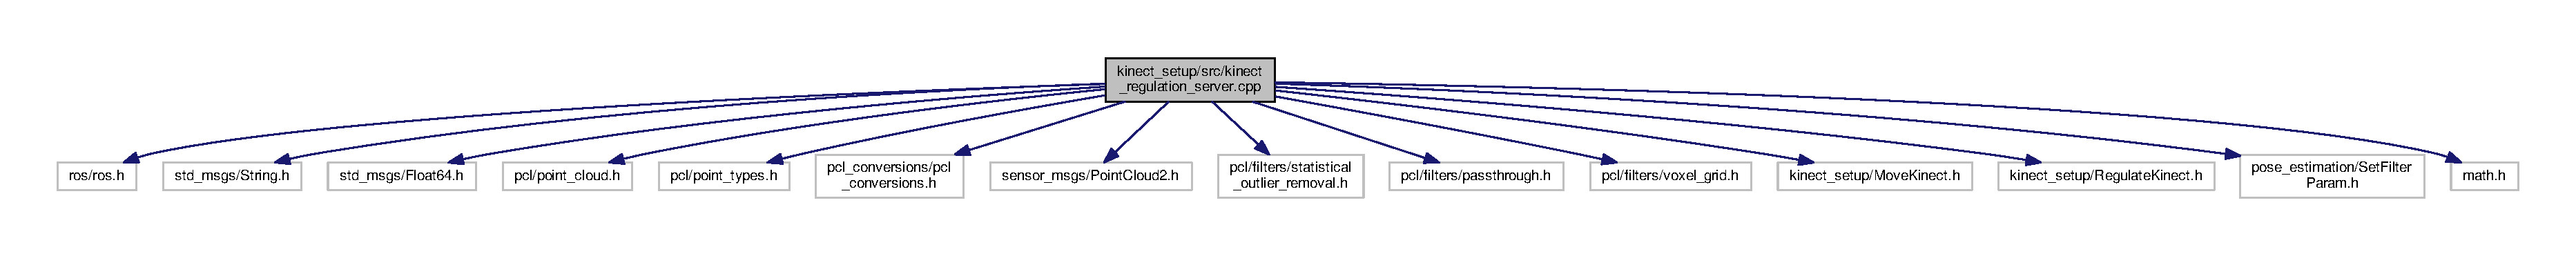
\includegraphics[width=350pt]{kinect__regulation__server_8cpp__incl}
\end{center}
\end{figure}
\subsection*{Functions}
\begin{DoxyCompactItemize}
\item 
bool {\bfseries regulate} (kinect\+\_\+setup\+::\+Regulate\+Kinect\+::\+Request \&req, kinect\+\_\+setup\+::\+Regulate\+Kinect\+::\+Response \&res)\hypertarget{kinect__regulation__server_8cpp_a04a147a7f20c408ad46289d2d3f8c14d}{}\label{kinect__regulation__server_8cpp_a04a147a7f20c408ad46289d2d3f8c14d}

\item 
\hyperlink{kinect__regulation__server_8cpp_a5ea466849f21e6c2be4ef9b2eb8868d3}{main} (int argc, char $\ast$$\ast$argv)
\end{DoxyCompactItemize}
\subsection*{Variables}
\begin{DoxyCompactItemize}
\item 
ros\+::\+Publisher \hyperlink{kinect__regulation__server_8cpp_abce76e70ebfd7c17e73a477ff47a485e}{rec\+\_\+pub}
\item 
ros\+::\+Service\+Client \hyperlink{kinect__regulation__server_8cpp_a1fdaee71ea7131695e608c338b5ee833}{client\+\_\+move}
\begin{DoxyCompactList}\small\item\em !!!!!!!!!!!! non necessario \end{DoxyCompactList}\item 
ros\+::\+Service\+Client \hyperlink{kinect__regulation__server_8cpp_a338b88518fb61d8831128a707d8f40a1}{client\+\_\+filter}
\end{DoxyCompactItemize}


\subsection{Detailed Description}
Callback of the /regulate\+\_\+kinect service
\begin{DoxyItemize}
\item control the tilt angle of the Kinect according to the coordinates xyz provided by the Beacon
\item regulate the parameters of the filters according to the coordinates xyz 
\begin{DoxyParams}[1]{Parameters}
\mbox{\tt in}  & {\em req} & Request Message \\
\hline
\mbox{\tt in}  & {\em req.\+x} & x-\/coordinate of the watch \\
\hline
\mbox{\tt in}  & {\em req.\+y} & y-\/coordinate of the watch \\
\hline
\mbox{\tt in}  & {\em req.\+z} & z-\/coordinate of the watch \\
\hline
\mbox{\tt out}  & {\em res} & Response of the service \\
\hline
\mbox{\tt out}  & {\em res.\+result} & If the operation is completed successfully \\
\hline
\end{DoxyParams}

\end{DoxyItemize}

\subsection{Function Documentation}
\index{kinect\+\_\+regulation\+\_\+server.\+cpp@{kinect\+\_\+regulation\+\_\+server.\+cpp}!main@{main}}
\index{main@{main}!kinect\+\_\+regulation\+\_\+server.\+cpp@{kinect\+\_\+regulation\+\_\+server.\+cpp}}
\subsubsection[{\texorpdfstring{main(int argc, char $\ast$$\ast$argv)}{main(int argc, char **argv)}}]{\setlength{\rightskip}{0pt plus 5cm}main (
\begin{DoxyParamCaption}
\item[{int}]{argc, }
\item[{char $\ast$$\ast$}]{argv}
\end{DoxyParamCaption}
)}\hypertarget{kinect__regulation__server_8cpp_a5ea466849f21e6c2be4ef9b2eb8868d3}{}\label{kinect__regulation__server_8cpp_a5ea466849f21e6c2be4ef9b2eb8868d3}
Main\+: Initialization of the service 

\subsection{Variable Documentation}
\index{kinect\+\_\+regulation\+\_\+server.\+cpp@{kinect\+\_\+regulation\+\_\+server.\+cpp}!client\+\_\+filter@{client\+\_\+filter}}
\index{client\+\_\+filter@{client\+\_\+filter}!kinect\+\_\+regulation\+\_\+server.\+cpp@{kinect\+\_\+regulation\+\_\+server.\+cpp}}
\subsubsection[{\texorpdfstring{client\+\_\+filter}{client_filter}}]{\setlength{\rightskip}{0pt plus 5cm}ros\+::\+Service\+Client client\+\_\+filter}\hypertarget{kinect__regulation__server_8cpp_a338b88518fb61d8831128a707d8f40a1}{}\label{kinect__regulation__server_8cpp_a338b88518fb61d8831128a707d8f40a1}
Client, to regulate the parameters of filters applied to the point cloud obtained by the background segmentation \index{kinect\+\_\+regulation\+\_\+server.\+cpp@{kinect\+\_\+regulation\+\_\+server.\+cpp}!client\+\_\+move@{client\+\_\+move}}
\index{client\+\_\+move@{client\+\_\+move}!kinect\+\_\+regulation\+\_\+server.\+cpp@{kinect\+\_\+regulation\+\_\+server.\+cpp}}
\subsubsection[{\texorpdfstring{client\+\_\+move}{client_move}}]{\setlength{\rightskip}{0pt plus 5cm}ros\+::\+Service\+Client client\+\_\+move}\hypertarget{kinect__regulation__server_8cpp_a1fdaee71ea7131695e608c338b5ee833}{}\label{kinect__regulation__server_8cpp_a1fdaee71ea7131695e608c338b5ee833}


!!!!!!!!!!!! non necessario 

Client, to control the tilt angle of the Kinect \index{kinect\+\_\+regulation\+\_\+server.\+cpp@{kinect\+\_\+regulation\+\_\+server.\+cpp}!rec\+\_\+pub@{rec\+\_\+pub}}
\index{rec\+\_\+pub@{rec\+\_\+pub}!kinect\+\_\+regulation\+\_\+server.\+cpp@{kinect\+\_\+regulation\+\_\+server.\+cpp}}
\subsubsection[{\texorpdfstring{rec\+\_\+pub}{rec_pub}}]{\setlength{\rightskip}{0pt plus 5cm}ros\+::\+Publisher rec\+\_\+pub}\hypertarget{kinect__regulation__server_8cpp_abce76e70ebfd7c17e73a477ff47a485e}{}\label{kinect__regulation__server_8cpp_abce76e70ebfd7c17e73a477ff47a485e}
Publisher, to control the tilt angle of the Kinect 
%--- End generated contents ---

% Index
\backmatter
\newpage
\phantomsection
\clearemptydoublepage
\addcontentsline{toc}{chapter}{Index}
\printindex

\end{document}
